Of the 461 images, 337 had a lesion mask that passed the checks (139 of 256 Derm7pt images and 198 of 205 PAD-UFES-20 images); tests (a) and (b) use these 337, and the other tests use all images. Both models answered every question. The tables below are generated by the analysis code directly from the per-image answers.

\subsection{Diagnosis on the original images}

MedGemma was more accurate than Qwen2.5-VL on both datasets (Table~\ref{tab:baseline}), and both were well above chance but far from useful as a diagnostic tool. Both models over-called melanoma: it was the forced-choice answer for 52\% (MedGemma) and 53\% (Qwen2.5-VL) of the original images, although only 20\% of the sampled lesions were melanomas. Qwen2.5-VL chose ``cannot be determined'' much more often, especially on the smartphone photographs (81.0\%).

\begin{table}[H]\centering\small
\caption{Diagnosis on the original images, forced choice among 8 diagnoses (\%, 95\% bootstrap interval). Chance balanced accuracy is 12.5\%.}\label{tab:baseline}
\begin{tabular}{lcc}\toprule
 & MedGemma 1.5 4B & Qwen2.5-VL 3B \\\midrule
\textit{derm7pt} ($n=256$) &  &  \\
\quad Accuracy & 33.2 (27.3--39.1) & 27.7 (21.9--33.2) \\
\quad Balanced accuracy & 28.0 (23.8--32.0) & 20.9 (18.2--23.9) \\
\quad Answered ``cannot be determined'' & 9.0 & 30.5 \\
\textit{pad} ($n=205$) &  &  \\
\quad Accuracy & 42.4 (36.1--49.3) & 27.8 (21.5--34.1) \\
\quad Balanced accuracy & 43.4 (38.7--48.4) & 27.7 (21.9--33.5) \\
\quad Answered ``cannot be determined'' & 29.8 & 81.0 \\
\bottomrule\end{tabular}\end{table}

\begin{table}[H]\centering\small
\caption{Test (a): the lesion is painted over with surrounding skin (\%). A confident diagnosis means not answering ``cannot be determined'' and giving the top diagnosis at least 50\% probability.}\label{tab:removed}
\begin{tabular}{lcc}\toprule
 & MedGemma 1.5 4B & Qwen2.5-VL 3B \\\midrule
Images & 337 & 337 \\
``Cannot be determined'', original & 18.4 (14.2--22.6) & 59.9 (54.6--65.0) \\
``Cannot be determined'', lesion removed & 48.1 (42.7--53.1) & 96.7 (94.7--98.5) \\
Confident diagnosis with lesion removed & 50.7 (45.7--56.1) & 2.4 (0.9--4.2) \\
Same diagnosis as on the original & 32.6 (27.6--37.7) & 30.3 (25.5--35.6) \\
Accuracy, original $\rightarrow$ lesion removed & 39.5 $\rightarrow$ 28.8 & 29.1 $\rightarrow$ 15.7 \\
\bottomrule\end{tabular}\end{table}

\begin{table}[H]\centering\small
\caption{Test (b): only the skin around the lesion is changed; lesion pixels are identical (\%, 95\% bootstrap interval).}\label{tab:background}
\begin{tabular}{lcc}\toprule
 & MedGemma 1.5 4B & Qwen2.5-VL 3B \\\midrule
\textit{Darker skin} &  &  \\
\quad Diagnosis changed & 13.4 (9.8--17.2) & 29.1 (24.3--34.1) \\
\quad Change in P(melanoma), points & +0.7 (-0.7 to +2.1) & +2.3 (+1.2 to +3.4) \\
\textit{Skin marker} &  &  \\
\quad Diagnosis changed & 10.1 (7.1--13.4) & 23.7 (19.3--28.2) \\
\quad Change in P(melanoma), points & -0.1 (-1.0 to +0.8) & +0.7 (-0.2 to +1.5) \\
\textit{Ruler} &  &  \\
\quad Diagnosis changed & 6.2 (3.9--8.9) & 19.0 (14.8--23.1) \\
\quad Change in P(melanoma), points & +1.9 (+1.1 to +2.8) & +1.1 (+0.4 to +1.8) \\
\bottomrule\end{tabular}\end{table}

\begin{table}[H]\centering\small
\caption{Test (c): AUROC of the model's yes-probability for each 7-point checklist criterion against the Derm7pt expert label (95\% bootstrap interval; 0.5 is chance). Prevalence in brackets.}\label{tab:criteria}
\begin{tabular}{lcc}\toprule
 & MedGemma 1.5 4B & Qwen2.5-VL 3B \\\midrule
atypical network (17\%) & 0.81 (0.74--0.86) & 0.67 (0.58--0.75) \\
blue white veil (20\%) & 0.84 (0.79--0.89) & 0.74 (0.66--0.82) \\
atypical vascular (5\%) & 0.62 (0.45--0.76) & 0.66 (0.52--0.80) \\
irregular streaks (20\%) & 0.75 (0.69--0.82) & 0.59 (0.50--0.67) \\
irregular pigmentation (33\%) & 0.77 (0.71--0.83) & 0.59 (0.51--0.66) \\
irregular dots (46\%) & 0.62 (0.56--0.69) & 0.55 (0.48--0.63) \\
regression (20\%) & 0.52 (0.44--0.61) & 0.46 (0.37--0.54) \\
\bottomrule\end{tabular}\end{table}

\begin{table}[H]\centering\small
\caption{Test (d): calibration on the original images (expected calibration error, 10 bins).}\label{tab:calibration}
\begin{tabular}{lcc}\toprule
 & MedGemma 1.5 4B & Qwen2.5-VL 3B \\\midrule
\textit{derm7pt} &  &  \\
\quad Accuracy / mean token confidence & 33.2 / 68.3 & 27.7 / 51.1 \\
\quad Token ECE & 0.35 (0.29--0.41) & 0.23 (0.18--0.29) \\
\quad Verbal ECE (answers naming a diagnosis) & 0.61 (0.55--0.67) (242/256) & 0.53 (0.36--0.68) (36/256) \\
\textit{pad} &  &  \\
\quad Accuracy / mean token confidence & 42.4 / 80.6 & 27.8 / 32.7 \\
\quad Token ECE & 0.39 (0.32--0.45) & 0.08 (0.05--0.14) \\
\quad Verbal ECE (answers naming a diagnosis) & 0.45 (0.37--0.52) (156/205) & 0.67 (0.46--0.84) (19/205) \\
\bottomrule\end{tabular}\end{table}


\subsection{(a) Lesion removed}

The two models behaved very differently when the lesion was painted out (Table~\ref{tab:removed}, Figure~\ref{fig:removed}). Qwen2.5-VL answered ``cannot be determined'' for 96.7\% of these images and gave a confident diagnosis for only 2.4\%. MedGemma abstained for 48.1\% and gave a confident diagnosis for 50.7\%; its mean confidence in its top diagnosis fell only from 75.7\% to 70.4\%. With the lesion removed, MedGemma's answer was usually ``nevus'' (71\% of Derm7pt images and 52\% of PAD-UFES-20 images, where ``basal cell carcinoma'' made up most of the rest). Its accuracy on Derm7pt images without a lesion (35.3\%) was close to what always answering ``nevus'' would give in that subset (30.2\%), so the remaining accuracy reflects a default answer rather than information in the surrounding skin.

\begin{figure}[H]\centering
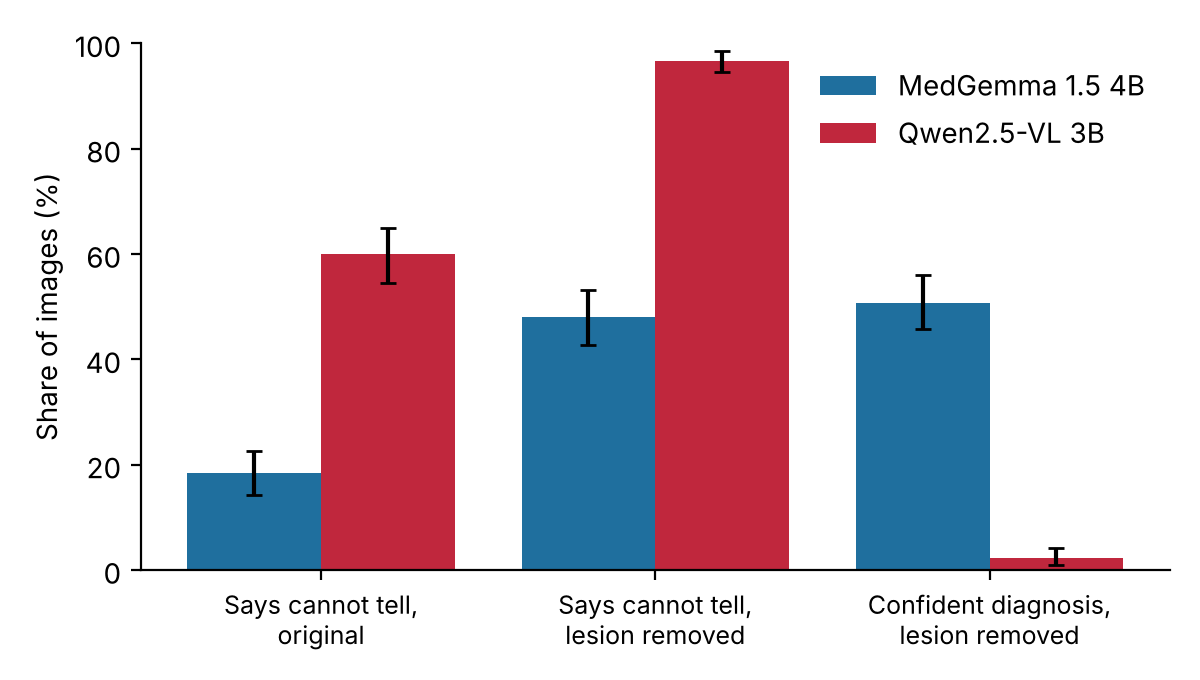
\includegraphics[width=0.72\textwidth]{lesion_removed.png}
\caption{Test (a). Share of images on which each model answers ``cannot be determined'', before and after the lesion is painted out, and share on which it still gives a confident diagnosis (top probability at least 50\%). 95\% bootstrap intervals; $n=337$.}\label{fig:removed}
\end{figure}

\subsection{(b) Background changed, lesion unchanged}

Every background edit changed some diagnoses even though the lesion pixels were identical (Table~\ref{tab:background}, Figure~\ref{fig:background}). Qwen2.5-VL was the less stable model: 29.1\% of its diagnoses changed when the surrounding skin was darkened, 23.7\% with skin-marker lines and 19.0\% with a ruler. For MedGemma the figures were 13.4\%, 10.1\% and 6.2\%. The edits moved the probability of melanoma only slightly on average. The clearest effects were a ruler raising MedGemma's probability of melanoma by 1.9 points (95\% CI 1.1--2.8) and darker skin raising Qwen2.5-VL's by 2.3 points (1.2--3.4); skin-marker lines did not move either model's melanoma probability measurably. Accuracy changed little, which means the changed diagnoses were mostly swaps between wrong answers or between a right and a wrong one in both directions.

\begin{figure}[H]\centering
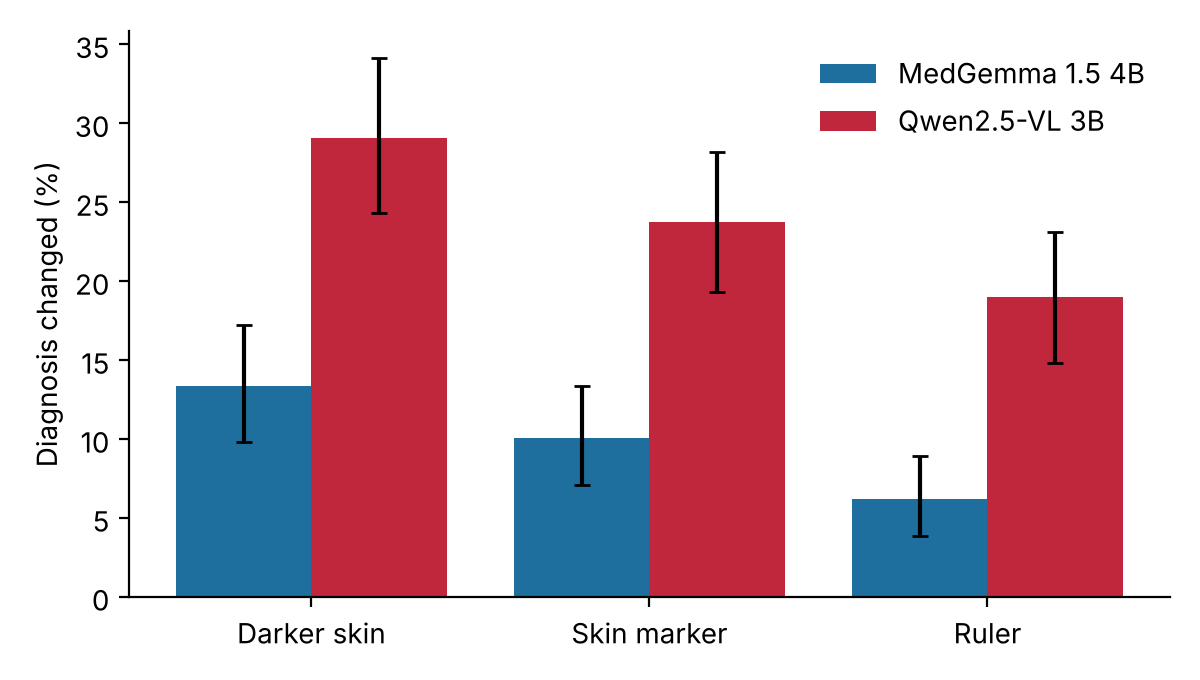
\includegraphics[width=0.66\textwidth]{background_flips.png}
\caption{Test (b). Share of images whose forced-choice diagnosis changed after an edit that left the lesion pixels untouched. 95\% bootstrap intervals; $n=337$ per edit.}\label{fig:background}
\end{figure}

\subsection{(c) Stated features}

MedGemma's answers on the seven checklist criteria matched the expert labels better than Qwen2.5-VL's for six of the seven criteria (Table~\ref{tab:criteria}, Figure~\ref{fig:criteria}); its best were blue-whitish veil (AUROC 0.84) and atypical pigment network (0.81). Regression structures were not recognised by either model (0.52 and 0.46). Both models said ``yes'' far more often than the criteria occur: Qwen2.5-VL said yes to irregular dots or globules for every image and to irregular pigmentation and atypical network for 99\%, while their prevalence was 47\%, 33\% and 17\%. A model's own checklist was linked to its own diagnosis much more strongly for MedGemma (Spearman correlation between the summed criterion probabilities and its melanoma probability 0.71) than for Qwen2.5-VL (0.25).

\begin{figure}[H]\centering
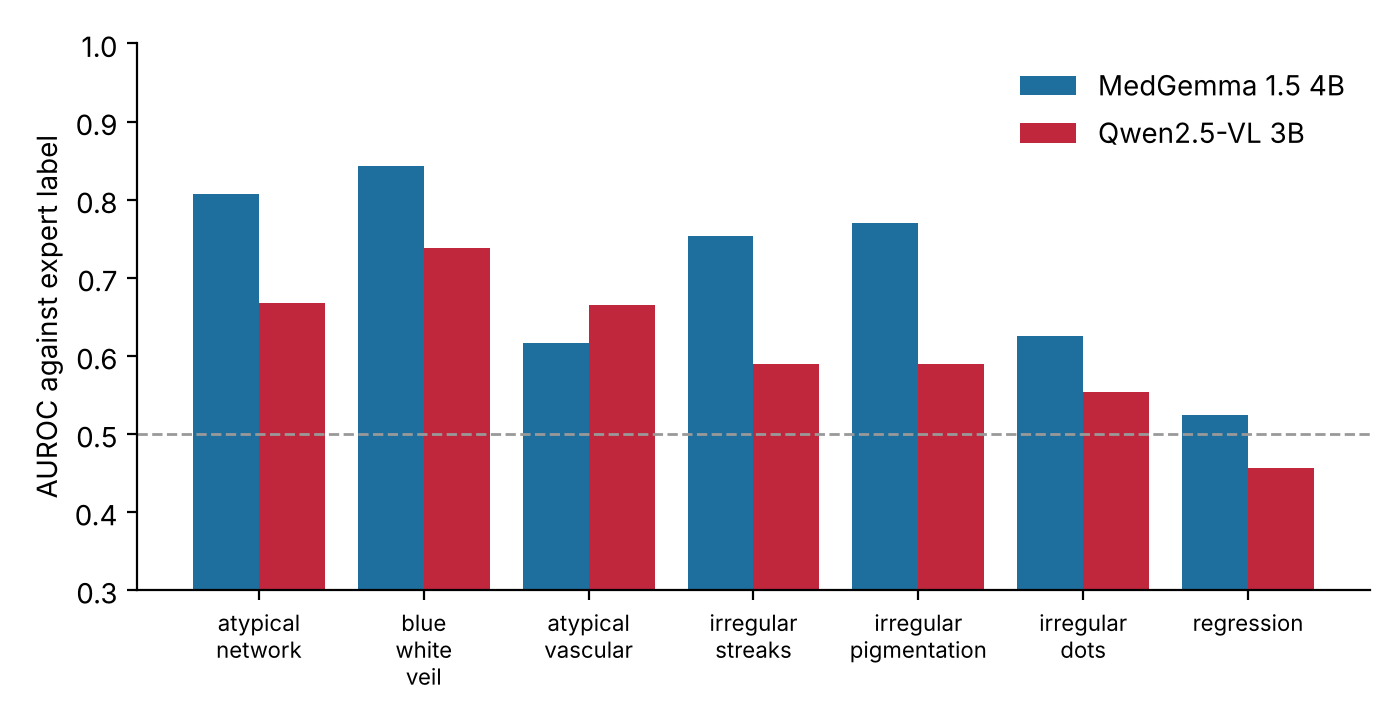
\includegraphics[width=0.72\textwidth]{criteria_auroc.png}
\caption{Test (c). AUROC of each model's yes-probability against the Derm7pt expert label for the seven criteria of the 7-point checklist ($n=256$). The dashed line is chance.}\label{fig:criteria}
\end{figure}

\subsection{(d) Calibration}

MedGemma was strongly overconfident (Table~\ref{tab:calibration}, Figure~\ref{fig:reliability}): its mean token confidence was 68.3\% on Derm7pt and 80.6\% on PAD-UFES-20, against accuracies of 33.2\% and 42.4\% (ECE 0.35 and 0.39). Qwen2.5-VL was overconfident on Derm7pt (51.1\% against 27.7\%, ECE 0.23) but close to calibrated on PAD-UFES-20 (ECE 0.08), where it was rarely confident at all. Confidence stated in words was worse for both models. MedGemma named a diagnosis in its free-text answer for 242 of 256 Derm7pt and 156 of 205 PAD-UFES-20 images, with ECE 0.61 and 0.45; Qwen2.5-VL named one for only 36 and 19 images, so its verbal calibration rests on very few answers.

\begin{figure}[H]\centering
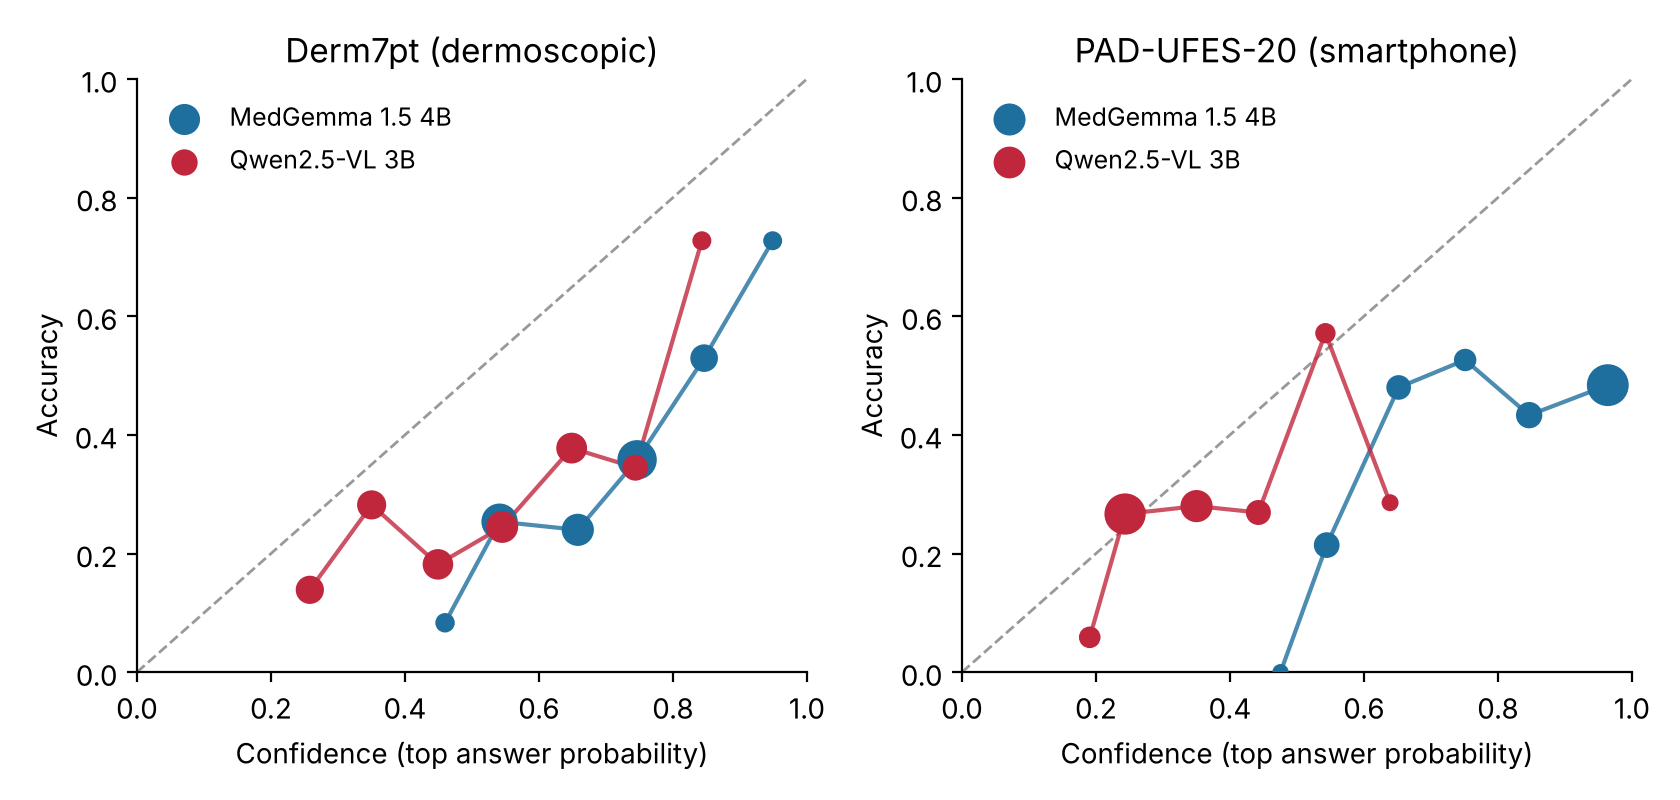
\includegraphics[width=0.9\textwidth]{reliability.png}
\caption{Test (d). Reliability diagrams for the token confidence on the original images; marker size shows the number of images in a bin, and bins with fewer than five images are not drawn. A calibrated model lies on the dashed line.}\label{fig:reliability}
\end{figure}
